%%%%%%%%%%%%%%%%%%%%%%%%%%%%%%%%%%%%%%%%%%%%%%%%%%%%%%%%%%%%%%%%%%%%%%%%%%%%%%
\section{Optimization of the degrader geometry}

\begin{itemize}
\item 
  For \piplusenu\ select tracks with small impact parameters.
\item 
  Expect muon decays in flight with muons far from the beam axis to be suppressed
  by the impact parameter selection.
\item
  therefore, can reduce the radius of the lead part down to what ? - try 
\end{itemize}

%%%%%%%%%%%%%%%%%%%%%%%%%%%%%%%%%%%%%%%%%%%%%%%%%%%%%%%%%%%%%%%%%%%%%%%%%%%%%%
\subsection{Converter position in Z}

\begin{itemize}
\item
  compare converter positioned at the same Z as the polyethylene disk
  to converter moved forward by 1cm 
\end{itemize}

%%%%%%%%%%%%%%%%%%%%%%%%%%%%%%%%%%%%%%%%%%%%%%%%%%%%%%%%%%%%%%%%%%%%%%%%%%%%%%
\subsection{Converter thickness - connection to \piplusenu\  calibration}

\begin{figure}[H]
  \begin{tikzpicture}
    \node[anchor=south west,inner sep=0] at (0,0.) {
      % \node[shift={(0 cm,0.cm)},inner sep=0,rotate={90}] at (0,0) {}
      \makebox[\textwidth][c] {
        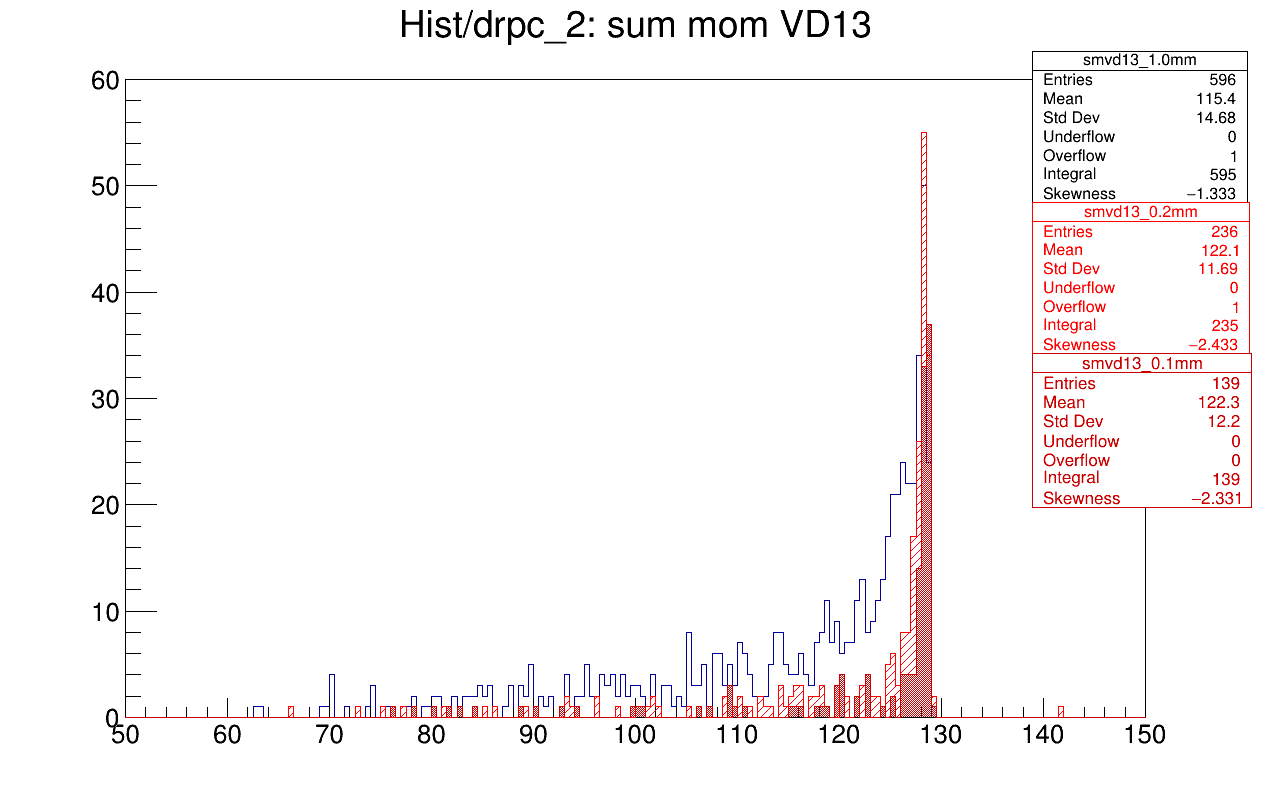
\includegraphics[width=0.9\textwidth]{png/sum_mom_vd13_001}
      }
    };
    % \node [text width=8cm, scale=1.0] at (14.5,0.5) {$\mu_B$, expected background mean};
    % \node [text width=8cm, scale=1.0, rotate={90}] at (1.5,7.5) { $S_{D}$, ``discovery'' signal strength  };
  \end{tikzpicture}
  \caption{
    \label{figure:sum_mom_vd13}
    momentum scheme calibration
  }
\end{figure}

The converter thickness is chosen based on the distributions shown in Figure~\ref{figure:sum_mom_vd13}.
Plotted: $P_{tot} = P_1 + P_2$ at VD13, virtual detector in front of the tracker fro events with
two particles, an electron and a positron with P > 30 MeV/c and producing 20 or more straw hits in the tracker each.
Such particles provide a good proxy to the reconstructable tracks.

The event yield increases with the converter thickness. However of interest for the scale calibration only
are the events close to the kinematic edge.
The highest yield of events with P > 128 Mev/c corresponds to the 100 um gold foil, and that determines
the choice of 100 um thick converter.

%%% Local Variables:
%%% mode: latex
%%% TeX-master: t
%%% End:
